\documentclass[]{article}
\usepackage{lmodern}
\usepackage{amssymb,amsmath}
\usepackage{ifxetex,ifluatex}
\usepackage{fixltx2e} % provides \textsubscript
\ifnum 0\ifxetex 1\fi\ifluatex 1\fi=0 % if pdftex
  \usepackage[T1]{fontenc}
  \usepackage[utf8]{inputenc}
\else % if luatex or xelatex
  \ifxetex
    \usepackage{mathspec}
  \else
    \usepackage{fontspec}
  \fi
  \defaultfontfeatures{Ligatures=TeX,Scale=MatchLowercase}
\fi
% use upquote if available, for straight quotes in verbatim environments
\IfFileExists{upquote.sty}{\usepackage{upquote}}{}
% use microtype if available
\IfFileExists{microtype.sty}{%
\usepackage[]{microtype}
\UseMicrotypeSet[protrusion]{basicmath} % disable protrusion for tt fonts
}{}
\PassOptionsToPackage{hyphens}{url} % url is loaded by hyperref
\usepackage[unicode=true]{hyperref}
\hypersetup{
            pdftitle={Air Quality in Southampton (UK)},
            pdfauthor={Ben Anderson (b.anderson@soton.ac.uk @dataknut)},
            pdfborder={0 0 0},
            breaklinks=true}
\urlstyle{same}  % don't use monospace font for urls
\usepackage[margin=1in]{geometry}
\usepackage{color}
\usepackage{fancyvrb}
\newcommand{\VerbBar}{|}
\newcommand{\VERB}{\Verb[commandchars=\\\{\}]}
\DefineVerbatimEnvironment{Highlighting}{Verbatim}{commandchars=\\\{\}}
% Add ',fontsize=\small' for more characters per line
\usepackage{framed}
\definecolor{shadecolor}{RGB}{248,248,248}
\newenvironment{Shaded}{\begin{snugshade}}{\end{snugshade}}
\newcommand{\KeywordTok}[1]{\textcolor[rgb]{0.13,0.29,0.53}{\textbf{#1}}}
\newcommand{\DataTypeTok}[1]{\textcolor[rgb]{0.13,0.29,0.53}{#1}}
\newcommand{\DecValTok}[1]{\textcolor[rgb]{0.00,0.00,0.81}{#1}}
\newcommand{\BaseNTok}[1]{\textcolor[rgb]{0.00,0.00,0.81}{#1}}
\newcommand{\FloatTok}[1]{\textcolor[rgb]{0.00,0.00,0.81}{#1}}
\newcommand{\ConstantTok}[1]{\textcolor[rgb]{0.00,0.00,0.00}{#1}}
\newcommand{\CharTok}[1]{\textcolor[rgb]{0.31,0.60,0.02}{#1}}
\newcommand{\SpecialCharTok}[1]{\textcolor[rgb]{0.00,0.00,0.00}{#1}}
\newcommand{\StringTok}[1]{\textcolor[rgb]{0.31,0.60,0.02}{#1}}
\newcommand{\VerbatimStringTok}[1]{\textcolor[rgb]{0.31,0.60,0.02}{#1}}
\newcommand{\SpecialStringTok}[1]{\textcolor[rgb]{0.31,0.60,0.02}{#1}}
\newcommand{\ImportTok}[1]{#1}
\newcommand{\CommentTok}[1]{\textcolor[rgb]{0.56,0.35,0.01}{\textit{#1}}}
\newcommand{\DocumentationTok}[1]{\textcolor[rgb]{0.56,0.35,0.01}{\textbf{\textit{#1}}}}
\newcommand{\AnnotationTok}[1]{\textcolor[rgb]{0.56,0.35,0.01}{\textbf{\textit{#1}}}}
\newcommand{\CommentVarTok}[1]{\textcolor[rgb]{0.56,0.35,0.01}{\textbf{\textit{#1}}}}
\newcommand{\OtherTok}[1]{\textcolor[rgb]{0.56,0.35,0.01}{#1}}
\newcommand{\FunctionTok}[1]{\textcolor[rgb]{0.00,0.00,0.00}{#1}}
\newcommand{\VariableTok}[1]{\textcolor[rgb]{0.00,0.00,0.00}{#1}}
\newcommand{\ControlFlowTok}[1]{\textcolor[rgb]{0.13,0.29,0.53}{\textbf{#1}}}
\newcommand{\OperatorTok}[1]{\textcolor[rgb]{0.81,0.36,0.00}{\textbf{#1}}}
\newcommand{\BuiltInTok}[1]{#1}
\newcommand{\ExtensionTok}[1]{#1}
\newcommand{\PreprocessorTok}[1]{\textcolor[rgb]{0.56,0.35,0.01}{\textit{#1}}}
\newcommand{\AttributeTok}[1]{\textcolor[rgb]{0.77,0.63,0.00}{#1}}
\newcommand{\RegionMarkerTok}[1]{#1}
\newcommand{\InformationTok}[1]{\textcolor[rgb]{0.56,0.35,0.01}{\textbf{\textit{#1}}}}
\newcommand{\WarningTok}[1]{\textcolor[rgb]{0.56,0.35,0.01}{\textbf{\textit{#1}}}}
\newcommand{\AlertTok}[1]{\textcolor[rgb]{0.94,0.16,0.16}{#1}}
\newcommand{\ErrorTok}[1]{\textcolor[rgb]{0.64,0.00,0.00}{\textbf{#1}}}
\newcommand{\NormalTok}[1]{#1}
\usepackage{longtable,booktabs}
% Fix footnotes in tables (requires footnote package)
\IfFileExists{footnote.sty}{\usepackage{footnote}\makesavenoteenv{long table}}{}
\usepackage{graphicx,grffile}
\makeatletter
\def\maxwidth{\ifdim\Gin@nat@width>\linewidth\linewidth\else\Gin@nat@width\fi}
\def\maxheight{\ifdim\Gin@nat@height>\textheight\textheight\else\Gin@nat@height\fi}
\makeatother
% Scale images if necessary, so that they will not overflow the page
% margins by default, and it is still possible to overwrite the defaults
% using explicit options in \includegraphics[width, height, ...]{}
\setkeys{Gin}{width=\maxwidth,height=\maxheight,keepaspectratio}
\IfFileExists{parskip.sty}{%
\usepackage{parskip}
}{% else
\setlength{\parindent}{0pt}
\setlength{\parskip}{6pt plus 2pt minus 1pt}
}
\setlength{\emergencystretch}{3em}  % prevent overfull lines
\providecommand{\tightlist}{%
  \setlength{\itemsep}{0pt}\setlength{\parskip}{0pt}}
\setcounter{secnumdepth}{5}
% Redefines (sub)paragraphs to behave more like sections
\ifx\paragraph\undefined\else
\let\oldparagraph\paragraph
\renewcommand{\paragraph}[1]{\oldparagraph{#1}\mbox{}}
\fi
\ifx\subparagraph\undefined\else
\let\oldsubparagraph\subparagraph
\renewcommand{\subparagraph}[1]{\oldsubparagraph{#1}\mbox{}}
\fi

% set default figure placement to htbp
\makeatletter
\def\fps@figure{htbp}
\makeatother

\usepackage{etoolbox}
\makeatletter
\providecommand{\subtitle}[1]{% add subtitle to \maketitle
  \apptocmd{\@title}{\par {\large #1 \par}}{}{}
}
\makeatother

\title{Air Quality in Southampton (UK)}
\providecommand{\subtitle}[1]{}
\subtitle{Exploring the effect of UK covid 19 lockdown on air quality: Summary for
BBC South}
\author{Ben Anderson
(\href{mailto:b.anderson@soton.ac.uk}{\nolinkurl{b.anderson@soton.ac.uk}}
\texttt{@dataknut})}
\date{Last run at: 2020-06-18 21:52:53 (Europe/London)}

\begin{document}
\maketitle

{
\setcounter{tocdepth}{2}
\tableofcontents
}
\section{Introduction}\label{introduction}

This report describes exploratory analysis of changes in air quality in
the City of Southampton, UK in Spring 2020.

\begin{Shaded}
\begin{Highlighting}[]
\NormalTok{lastHA <-}\StringTok{ }\KeywordTok{max}\NormalTok{(fixedDT[source }\OperatorTok{==}\StringTok{ "hantsAir"}\NormalTok{]}\OperatorTok{$}\NormalTok{dateTimeUTC)}
\NormalTok{diffHA <-}\StringTok{ }\NormalTok{lubridate}\OperatorTok{::}\KeywordTok{now}\NormalTok{() }\OperatorTok{-}\StringTok{ }\NormalTok{lastHA}
\NormalTok{lastAURN <-}\StringTok{ }\KeywordTok{max}\NormalTok{(fixedDT[source }\OperatorTok{==}\StringTok{ "AURN"}\NormalTok{]}\OperatorTok{$}\NormalTok{dateTimeUTC)}
\NormalTok{diffAURN <-}\StringTok{ }\NormalTok{lubridate}\OperatorTok{::}\KeywordTok{now}\NormalTok{() }\OperatorTok{-}\StringTok{ }\NormalTok{lastAURN}
\end{Highlighting}
\end{Shaded}

Data for Southampton downloaded from :

\begin{itemize}
\tightlist
\item
  \url{http://www.hantsair.org.uk/hampshire/asp/Bulletin.asp?la=Southampton}
  (see also
  \url{https://www.southampton.gov.uk/environmental-issues/pollution/air-quality/});
\item
  \url{https://uk-air.defra.gov.uk/networks/network-info?view=aurn}
\end{itemize}

Southampton City Council collects various forms of air quality data at
the sites shown in Table @ref(tab:showSites). The data is available in
raw form from
\url{http://www.hantsair.org.uk/hampshire/asp/Bulletin.asp?la=Southampton\&bulletin=daily\&site=SH5}.

Some of these sites feed data to
\href{https://uk-air.defra.gov.uk/networks/network-info?view=aurn}{AURN}.
The data that goes via AURN is
\href{https://uk-air.defra.gov.uk/assets/documents/Data_Validation_and_Ratification_Process_Apr_2017.pdf}{ratified}
to check for outliers and instrument/measurement error. AURN data less
than six months old has not undergone this process. AURN data is (c)
Crown 2020 copyright Defra and available for re-use via
\url{https://uk-air.defra.gov.uk}, licenced under the
\href{http://www.nationalarchives.gov.uk/doc/open-government-licence/version/2/}{Open
Government Licence} (OGL).

\section{Data}\label{data}

In this report we use data from the following sources:

\begin{itemize}
\tightlist
\item
  \url{http://www.hantsair.org.uk/hampshire/asp/Bulletin.asp?la=Southampton}
  last updated at 2020-06-08 10:00:00;
\item
  \url{https://uk-air.defra.gov.uk/networks/network-info?view=aurn} last
  updated at 2020-06-07 23:00:00.
\end{itemize}

Table @ref(tab:showSites) shows the available sites and sources. Note
that some of the non-AURN sites appear to have stopped updating
recently. For a detailed analysis of recent missing data see Section
@ref(annexMissing).

\begin{Shaded}
\begin{Highlighting}[]
\NormalTok{t <-}\StringTok{ }\NormalTok{fixedDT[}\OperatorTok{!}\KeywordTok{is.na}\NormalTok{(value), .(}\DataTypeTok{nObs =}\NormalTok{ .N, }\DataTypeTok{firstData =} \KeywordTok{min}\NormalTok{(dateTimeUTC), }\DataTypeTok{latestData =} \KeywordTok{max}\NormalTok{(dateTimeUTC), }\DataTypeTok{nMeasures =} \KeywordTok{uniqueN}\NormalTok{(pollutant)), }
\NormalTok{    keyby =}\StringTok{ }\NormalTok{.(site, source)]}

\NormalTok{kableExtra}\OperatorTok{::}\KeywordTok{kable}\NormalTok{(t, }\DataTypeTok{caption =} \StringTok{"Sites, data source and number of valid observations. note that measures includes wind speed and direction in the AURN sourced data"}\NormalTok{, }
    \DataTypeTok{digits =} \DecValTok{2}\NormalTok{) }\OperatorTok\StringTok{ }\KeywordTok{kable_styling}\NormalTok{()}
\end{Highlighting}
\end{Shaded}

(\#tab:showSites)Sites, data source and number of valid observations.
note that measures includes wind speed and direction in the AURN sourced
data

site

source

nObs

firstData

latestData

nMeasures

Southampton - A33 Roadside (near docks, AURN site)

hantsAir

85918

2017-01-01 00:00:00

2020-06-08 10:00:00

3

Southampton - Background (near city centre, AURN site)

hantsAir

162148

2017-01-25 11:00:00

2020-06-08 10:00:00

6

Southampton - Onslow Road (near RSH)

hantsAir

82232

2017-01-01 00:00:00

2020-04-15 07:00:00

3

Southampton - Victoria Road (Woolston)

hantsAir

60078

2017-01-01 00:00:00

2020-04-01 06:00:00

3

Southampton A33 (via AURN)

AURN

220010

2017-01-01 00:00:00

2020-06-07 23:00:00

8

Southampton Centre (via AURN)

AURN

343216

2017-01-01 00:00:00

2020-06-07 23:00:00

13

Table @ref(tab:showPollutants) shows the poillutants recorded at each
site.

\begin{Shaded}
\begin{Highlighting}[]
\NormalTok{t <-}\StringTok{ }\KeywordTok{with}\NormalTok{(fixedDT[}\OperatorTok{!}\KeywordTok{is.na}\NormalTok{(value)], }\KeywordTok{table}\NormalTok{(pollutant, site))}

\NormalTok{kableExtra}\OperatorTok{::}\KeywordTok{kable}\NormalTok{(t, }\DataTypeTok{caption =} \StringTok{"Sites, pollutant and number of valid observations"}\NormalTok{, }\DataTypeTok{digits =} \DecValTok{2}\NormalTok{) }\OperatorTok\StringTok{ }\KeywordTok{kable_styling}\NormalTok{()}
\end{Highlighting}
\end{Shaded}

(\#tab:showPollutants)Sites, pollutant and number of valid observations

Southampton - A33 Roadside (near docks, AURN site)

Southampton - Background (near city centre, AURN site)

Southampton - Onslow Road (near RSH)

Southampton - Victoria Road (Woolston)

Southampton A33 (via AURN)

Southampton Centre (via AURN)

no

29055

28702

27412

20026

29641

28657

no2

29020

28702

27408

20026

29640

28657

nox

0

22877

27412

20026

29640

28658

nv10

0

0

0

0

23208

21105

nv2.5

0

0

0

0

0

22627

o3

0

0

0

0

0

28645

pm10

27843

26124

0

0

25681

26180

pm2.5

0

27632

0

0

0

27702

so2

0

0

0

0

0

28261

sp2

0

28111

0

0

0

0

v10

0

0

0

0

23208

21105

v2.5

0

0

0

0

0

22627

wd

0

0

0

0

29496

29496

ws

0

0

0

0

29496

29496

To avoid confusion and `double counting', in the remainder of the
analysis we replace the Southampton AURN site data with the data for the
same site sourced via AURN as shown in Table @ref(tab:selectFinalSites).
This has the disadvantage that the data is slightly less up to date (see
Table @ref(tab:showSites)). As will be explained below in the
comparative analysis we will use only the AURN data to avoid missing
data issues.

\begin{Shaded}
\begin{Highlighting}[]
\NormalTok{fixedDT <-}\StringTok{ }\NormalTok{fixedDT[}\OperatorTok{!}\NormalTok{(site }\OperatorTok\StringTok{ "AURN site"}\NormalTok{)]}

\NormalTok{t <-}\StringTok{ }\NormalTok{fixedDT[}\OperatorTok{!}\KeywordTok{is.na}\NormalTok{(value), .(}\DataTypeTok{nObs =}\NormalTok{ .N, }\DataTypeTok{nPollutants =} \KeywordTok{uniqueN}\NormalTok{(pollutant), }\DataTypeTok{lastDate =} \KeywordTok{max}\NormalTok{(dateTimeUTC)), keyby =}\StringTok{ }\NormalTok{.(site, }
\NormalTok{    source)]}

\NormalTok{kableExtra}\OperatorTok{::}\KeywordTok{kable}\NormalTok{(t, }\DataTypeTok{caption =} \StringTok{"Sites, data source and number of valid observations"}\NormalTok{, }\DataTypeTok{digits =} \DecValTok{2}\NormalTok{) }\OperatorTok\StringTok{ }\KeywordTok{kable_styling}\NormalTok{()}
\end{Highlighting}
\end{Shaded}

(\#tab:selectFinalSites)Sites, data source and number of valid
observations

site

source

nObs

nPollutants

lastDate

Southampton - Onslow Road (near RSH)

hantsAir

82232

3

2020-04-15 07:00:00

Southampton - Victoria Road (Woolston)

hantsAir

60078

3

2020-04-01 06:00:00

Southampton A33 (via AURN)

AURN

220010

8

2020-06-07 23:00:00

Southampton Centre (via AURN)

AURN

343216

13

2020-06-07 23:00:00

We use this data to compare:

\begin{itemize}
\tightlist
\item
  pre and during-lockdown air quality measures
\item
  air quality measures during lockdown 2020 with average measures for
  the same time periods in the preceding 3 years (2017-2019)
\end{itemize}

It should be noted that air pollution levels in any given period of time
are highly dependent on the prevailing meteorological conditions. As a
result it can be very difficult to disentangle the affects of a
reduction in source strength from the affects of local surface
conditions. This is abundantly clear in the analysis which follows given
that the Easter weekend was forecast to have
\href{https://airqualitynews.com/2020/04/07/people-at-risk-from-coronavirus-warned-with-very-high-air-pollution-episode-predicted-for-uk/}{very
high import of pollution from Europe} and that the wind direction and
speed was highly variable across the lockdown period (see Figure
@ref(fig:recentWind)).

Further, air quality is not wholly driven by sources that lockdown might
suppress and indeed that suppression may lead to rebound affects. For
example we might expect more emissions due to increased domestic heating
during cooler lockdown periods. As a result the analysis presented below
must be considered a preliminary `before meteorological adjustment' and
`before controlling for other sources' analysis of the affect of
lockdown on air quality in Southampton.

For much more detailed analysis see a longer and very messy
\href{https://dataknut.github.io/airQual/sccAirQualExplore_Exploring\%20the\%20SSC\%20and\%20AURN\%20data.html}{data
report}.

\section{WHO air quality thresholds}\label{who-air-quality-thresholds}

A number of the following plots show the relevant WHO air quality
thresholds and limits. These are taken from:

\begin{itemize}
\tightlist
\item
  \url{https://www.who.int/news-room/fact-sheets/detail/ambient-(outdoor)-air-quality-and-health}
\end{itemize}

\section{Nitrogen Dioxide (no2)}\label{nitrogen-dioxide-no2}

\begin{Shaded}
\begin{Highlighting}[]
\NormalTok{yLab <-}\StringTok{ "Nitrogen Dioxide (ug/m3)"}
\NormalTok{no2dt <-}\StringTok{ }\NormalTok{fixedDT[pollutant }\OperatorTok{==}\StringTok{ "no2"}\NormalTok{]}
\end{Highlighting}
\end{Shaded}

Figure @ref(fig:theilSenNO2) shows the NO2 trend over time. Is lockdown
below trend?

\begin{Shaded}
\begin{Highlighting}[]
\NormalTok{no2dt[, }\StringTok{`}\DataTypeTok{:=}\StringTok{`}\NormalTok{(date, }\KeywordTok{as.Date}\NormalTok{(dateTimeUTC))]  }\CommentTok{# set date to date for this one}

\NormalTok{oaNO2 <-}\StringTok{ }\NormalTok{openair}\OperatorTok{::}\KeywordTok{TheilSen}\NormalTok{(no2dt[date }\OperatorTok{<}\StringTok{ }\KeywordTok{as.Date}\NormalTok{(}\StringTok{"2020-06-01"}\NormalTok{)], }\StringTok{"value"}\NormalTok{, }\DataTypeTok{ylab =} \StringTok{"NO2"}\NormalTok{, }\DataTypeTok{deseason =} \OtherTok{TRUE}\NormalTok{, }\DataTypeTok{xlab =} \StringTok{"Year"}\NormalTok{, }
    \DataTypeTok{date.format =} \StringTok{"%Y"}\NormalTok{, }\DataTypeTok{date.breaks =} \DecValTok{4}\NormalTok{)}
\end{Highlighting}
\end{Shaded}

\begin{verbatim}
## [1] "Taking bootstrap samples. Please wait."
\end{verbatim}

\begin{figure}
\centering
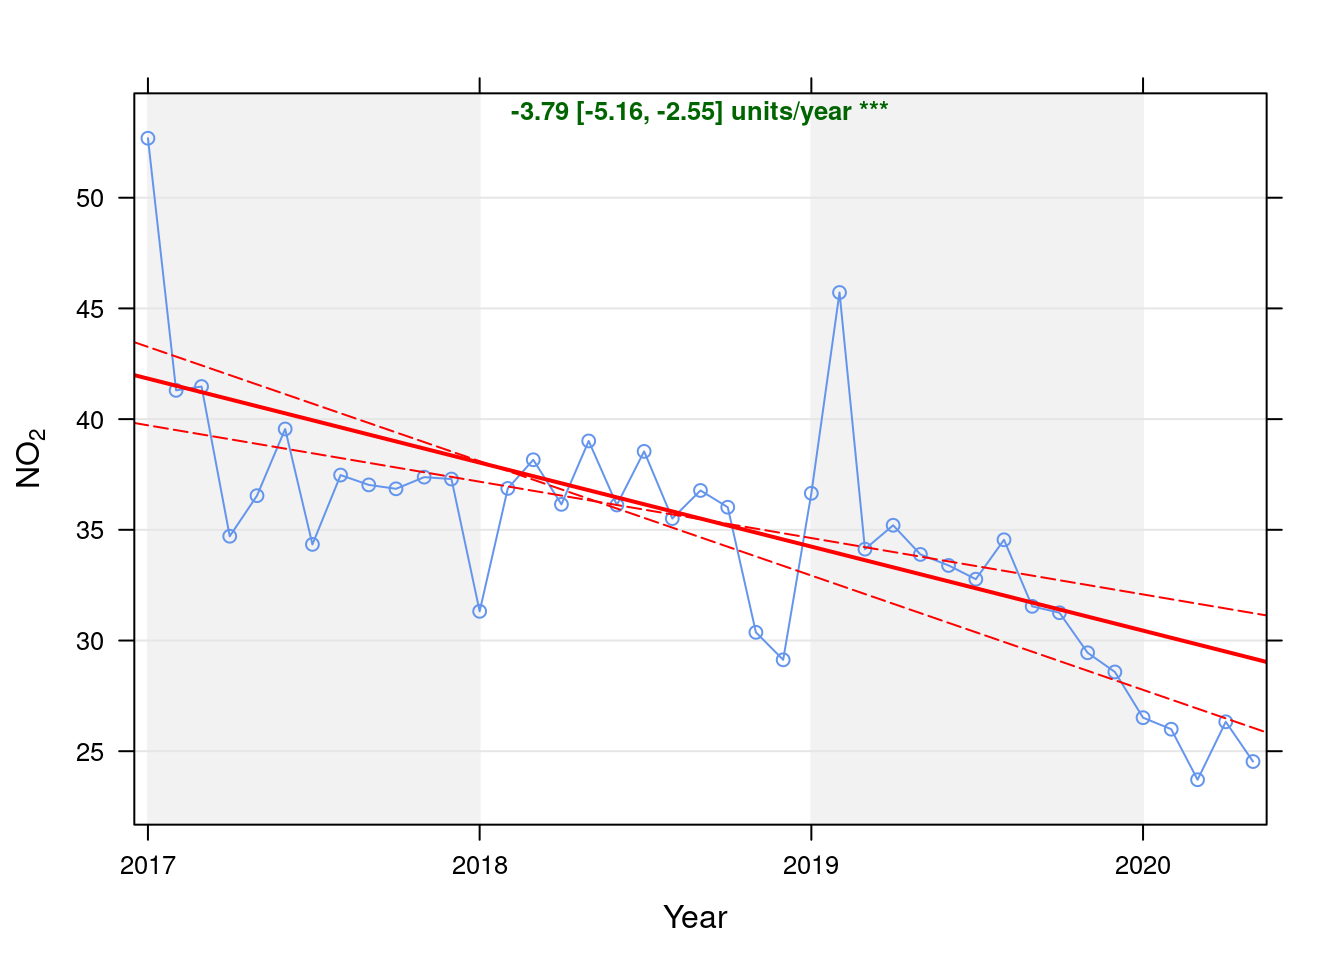
\includegraphics{/home/ba1e12/github/dataknut/airQual/docs/sccAirQualExplore_covidLockdown2020ForBBCsnaphot_files/figure-latex/theilSenNO2-1.pdf}
\caption{(\#fig:theilSenNO2)Theil-Sen trend (NO2)}
\end{figure}

\begin{Shaded}
\begin{Highlighting}[]
\NormalTok{p <-}\StringTok{ }\NormalTok{oaNO2}\OperatorTok{$}\NormalTok{plot}

\NormalTok{getModelTrendTable <-}\StringTok{ }\ControlFlowTok{function}\NormalTok{(oa, fname) \{}
    \CommentTok{# oa is an openAir object created by theilSen calculates the % below trend using the theil sen slope line}
    \CommentTok{# parameters oa <- oaGWh}
\NormalTok{    oaData <-}\StringTok{ }\KeywordTok{as.data.table}\NormalTok{(oa}\OperatorTok{$}\NormalTok{data}\OperatorTok{$}\NormalTok{main.data)}
\NormalTok{    rDT <-}\StringTok{ }\NormalTok{oaData[, .(date, conc, a, b, slope)]}
    \CommentTok{# https://github.com/davidcarslaw/openair/blob/master/R/TheilSen.R#L192 and}
    \CommentTok{# https://github.com/davidcarslaw/openair/blob/master/R/TheilSen.R#L625}
\NormalTok{    rDT[, }\StringTok{`}\DataTypeTok{:=}\StringTok{`}\NormalTok{(x, }\KeywordTok{time_length}\NormalTok{(date }\OperatorTok{-}\StringTok{ }\KeywordTok{as.Date}\NormalTok{(}\StringTok{"1970-01-01"}\NormalTok{), }\DataTypeTok{unit =} \StringTok{"days"}\NormalTok{))]  }\CommentTok{# n days since x = 0}
\NormalTok{    rDT[, }\StringTok{`}\DataTypeTok{:=}\StringTok{`}\NormalTok{(expectedVal, a }\OperatorTok{+}\StringTok{ }\NormalTok{(b }\OperatorTok{*}\StringTok{ }\NormalTok{x))]  }\CommentTok{# b = slope / 365}
    
    \CommentTok{# checks}
\NormalTok{    p <-}\StringTok{ }\NormalTok{ggplot2}\OperatorTok{::}\KeywordTok{ggplot}\NormalTok{(rDT, }\KeywordTok{aes}\NormalTok{(}\DataTypeTok{x =}\NormalTok{ date)) }\OperatorTok{+}\StringTok{ }\KeywordTok{geom_line}\NormalTok{(}\KeywordTok{aes}\NormalTok{(}\DataTypeTok{y =}\NormalTok{ conc)) }\OperatorTok{+}\StringTok{ }\KeywordTok{labs}\NormalTok{(}\DataTypeTok{y =} \StringTok{"Value"}\NormalTok{, }\DataTypeTok{caption =}\NormalTok{ fname)}
\NormalTok{    p <-}\StringTok{ }\NormalTok{p }\OperatorTok{+}\StringTok{ }\KeywordTok{geom_line}\NormalTok{(}\KeywordTok{aes}\NormalTok{(}\DataTypeTok{y =}\NormalTok{ expectedVal), }\DataTypeTok{linetype =} \StringTok{"dashed"}\NormalTok{)}
\NormalTok{    ggplot2}\OperatorTok{::}\KeywordTok{ggsave}\NormalTok{(here}\OperatorTok{::}\KeywordTok{here}\NormalTok{(}\StringTok{"docs"}\NormalTok{, }\StringTok{"plots"}\NormalTok{, }\KeywordTok{paste0}\NormalTok{(}\StringTok{"SSC_trendModelTestPlot_"}\NormalTok{, fname, }\StringTok{".png"}\NormalTok{)))}
\NormalTok{    rDT[, }\StringTok{`}\DataTypeTok{:=}\StringTok{`}\NormalTok{(diff, conc }\OperatorTok{-}\StringTok{ }\NormalTok{expectedVal)]}
\NormalTok{    rDT[, }\StringTok{`}\DataTypeTok{:=}\StringTok{`}\NormalTok{(pcDiff, (diff}\OperatorTok{/}\NormalTok{expectedVal) }\OperatorTok{*}\StringTok{ }\DecValTok{100}\NormalTok{)]}
    
\NormalTok{    t <-}\StringTok{ }\NormalTok{rDT[, .(date, conc, a, b, slope, expectedVal, diff, pcDiff)]}
    \KeywordTok{return}\NormalTok{(t)}
\NormalTok{\}}

\NormalTok{t <-}\StringTok{ }\KeywordTok{getModelTrendTable}\NormalTok{(oaNO2, }\DataTypeTok{fname =} \StringTok{"NO2"}\NormalTok{)}

\NormalTok{ft <-}\StringTok{ }\KeywordTok{dcast}\NormalTok{(t[date }\OperatorTok{>=}\StringTok{ }\KeywordTok{as.Date}\NormalTok{(}\StringTok{"2020-01-01"}\NormalTok{) }\OperatorTok{&}\StringTok{ }\NormalTok{date }\OperatorTok{<}\StringTok{ }\KeywordTok{as.Date}\NormalTok{(}\StringTok{"2020-06-01"}\NormalTok{)], date }\OperatorTok{~}\StringTok{ }\NormalTok{., }\DataTypeTok{value.var =} \KeywordTok{c}\NormalTok{(}\StringTok{"diff"}\NormalTok{, }\StringTok{"pcDiff"}\NormalTok{))}
\NormalTok{ft[, }\StringTok{`}\DataTypeTok{:=}\StringTok{`}\NormalTok{(date, }\KeywordTok{format.Date}\NormalTok{(date, }\DataTypeTok{format =} \StringTok{"%b %Y"}\NormalTok{))]}
\NormalTok{kableExtra}\OperatorTok{::}\KeywordTok{kable}\NormalTok{(ft, }\DataTypeTok{caption =} \StringTok{"Units and % above/below expected"}\NormalTok{, }\DataTypeTok{digits =} \DecValTok{2}\NormalTok{) }\OperatorTok\StringTok{ }\KeywordTok{kable_styling}\NormalTok{()}
\end{Highlighting}
\end{Shaded}

(\#tab:theilSenNO2)Units and \% above/below expected

date

diff

pcDiff

Jan 2020

-3.93

-12.91

Feb 2020

-4.13

-13.70

Mar 2020

-6.11

-20.49

Apr 2020

-3.17

-10.75

May 2020

-4.65

-15.94

\section{Oxides of Nitrogen (nox)}\label{oxides-of-nitrogen-nox}

\begin{Shaded}
\begin{Highlighting}[]
\NormalTok{yLab <-}\StringTok{ "Oxides of Nitrogen (ug/m3)"}
\NormalTok{noxdt <-}\StringTok{ }\NormalTok{fixedDT[pollutant }\OperatorTok{==}\StringTok{ "nox"}\NormalTok{]}
\end{Highlighting}
\end{Shaded}

Figure @ref(fig:theilSenNOx) shows the NOx trend over time. Is lockdown
below trend?

\begin{Shaded}
\begin{Highlighting}[]
\NormalTok{noxdt[, }\StringTok{`}\DataTypeTok{:=}\StringTok{`}\NormalTok{(date, }\KeywordTok{as.Date}\NormalTok{(dateTimeUTC))]  }\CommentTok{# set date to date for this one}

\NormalTok{oaNOx <-}\StringTok{ }\NormalTok{openair}\OperatorTok{::}\KeywordTok{TheilSen}\NormalTok{(noxdt[date }\OperatorTok{<}\StringTok{ }\KeywordTok{as.Date}\NormalTok{(}\StringTok{"2020-06-01"}\NormalTok{)], }\StringTok{"value"}\NormalTok{, }\DataTypeTok{ylab =} \StringTok{"NOx"}\NormalTok{, }\DataTypeTok{deseason =} \OtherTok{TRUE}\NormalTok{, }\DataTypeTok{xlab =} \StringTok{"Year"}\NormalTok{, }
    \DataTypeTok{date.format =} \StringTok{"%Y"}\NormalTok{, }\DataTypeTok{date.breaks =} \DecValTok{4}\NormalTok{)}
\end{Highlighting}
\end{Shaded}

\begin{verbatim}
## [1] "Taking bootstrap samples. Please wait."
\end{verbatim}

\begin{figure}
\centering
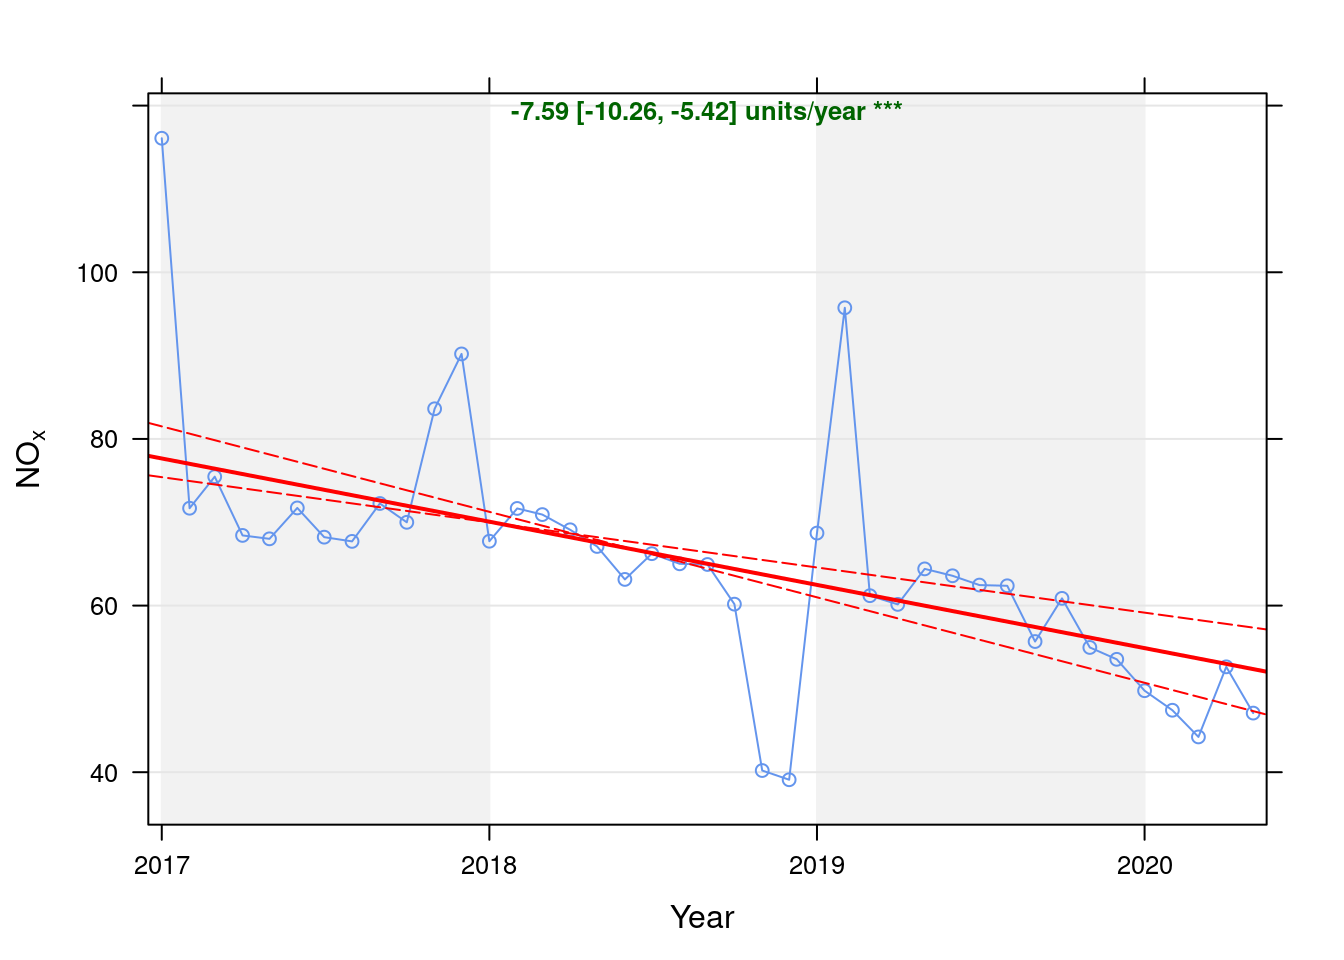
\includegraphics{/home/ba1e12/github/dataknut/airQual/docs/sccAirQualExplore_covidLockdown2020ForBBCsnaphot_files/figure-latex/theilSenNOx-1.pdf}
\caption{(\#fig:theilSenNOx)Theil-Sen trend (NOx)}
\end{figure}

\begin{Shaded}
\begin{Highlighting}[]
\NormalTok{p <-}\StringTok{ }\NormalTok{oaNOx}\OperatorTok{$}\NormalTok{plot}

\NormalTok{t <-}\StringTok{ }\KeywordTok{getModelTrendTable}\NormalTok{(oaNOx, }\DataTypeTok{fname =} \StringTok{"NOx"}\NormalTok{)}

\NormalTok{ft <-}\StringTok{ }\KeywordTok{dcast}\NormalTok{(t[date }\OperatorTok{>=}\StringTok{ }\KeywordTok{as.Date}\NormalTok{(}\StringTok{"2020-01-01"}\NormalTok{) }\OperatorTok{&}\StringTok{ }\NormalTok{date }\OperatorTok{<}\StringTok{ }\KeywordTok{as.Date}\NormalTok{(}\StringTok{"2020-06-01"}\NormalTok{)], date }\OperatorTok{~}\StringTok{ }\NormalTok{., }\DataTypeTok{value.var =} \KeywordTok{c}\NormalTok{(}\StringTok{"diff"}\NormalTok{, }\StringTok{"pcDiff"}\NormalTok{))}
\NormalTok{ft[, }\StringTok{`}\DataTypeTok{:=}\StringTok{`}\NormalTok{(date, }\KeywordTok{format.Date}\NormalTok{(date, }\DataTypeTok{format =} \StringTok{"%b %Y"}\NormalTok{))]}
\NormalTok{kableExtra}\OperatorTok{::}\KeywordTok{kable}\NormalTok{(ft, }\DataTypeTok{caption =} \StringTok{"Units and % above/below expected"}\NormalTok{, }\DataTypeTok{digits =} \DecValTok{2}\NormalTok{) }\OperatorTok\StringTok{ }\KeywordTok{kable_styling}\NormalTok{()}
\end{Highlighting}
\end{Shaded}

(\#tab:theilSenNOx)Units and \% above/below expected

date

diff

pcDiff

Jan 2020

-5.11

-9.30

Feb 2020

-6.81

-12.55

Mar 2020

-9.41

-17.54

Apr 2020

-0.35

-0.66

May 2020

-5.28

-10.08

\section{Sulphour Dioxide}\label{sulphour-dioxide}

\begin{Shaded}
\begin{Highlighting}[]
\NormalTok{yLab <-}\StringTok{ "Sulphour Dioxide (ug/m3)"}
\NormalTok{so2dt <-}\StringTok{ }\NormalTok{fixedDT[pollutant }\OperatorTok{==}\StringTok{ "so2"}\NormalTok{]}
\end{Highlighting}
\end{Shaded}

Figure @ref(fig:theilSenSO2) shows the SO2 trend over time. Is lockdown
below trend?

\begin{Shaded}
\begin{Highlighting}[]
\NormalTok{so2dt[, }\StringTok{`}\DataTypeTok{:=}\StringTok{`}\NormalTok{(date, }\KeywordTok{as.Date}\NormalTok{(dateTimeUTC))]  }\CommentTok{# set date to date for this one}

\NormalTok{oaSO2 <-}\StringTok{ }\NormalTok{openair}\OperatorTok{::}\KeywordTok{TheilSen}\NormalTok{(noxdt[date }\OperatorTok{<}\StringTok{ }\KeywordTok{as.Date}\NormalTok{(}\StringTok{"2020-06-01"}\NormalTok{)], }\StringTok{"value"}\NormalTok{, }\DataTypeTok{ylab =} \StringTok{"SO2"}\NormalTok{, }\DataTypeTok{deseason =} \OtherTok{TRUE}\NormalTok{, }\DataTypeTok{xlab =} \StringTok{"Year"}\NormalTok{, }
    \DataTypeTok{date.format =} \StringTok{"%Y"}\NormalTok{, }\DataTypeTok{date.breaks =} \DecValTok{4}\NormalTok{)}
\end{Highlighting}
\end{Shaded}

\begin{verbatim}
## [1] "Taking bootstrap samples. Please wait."
\end{verbatim}

\begin{figure}
\centering
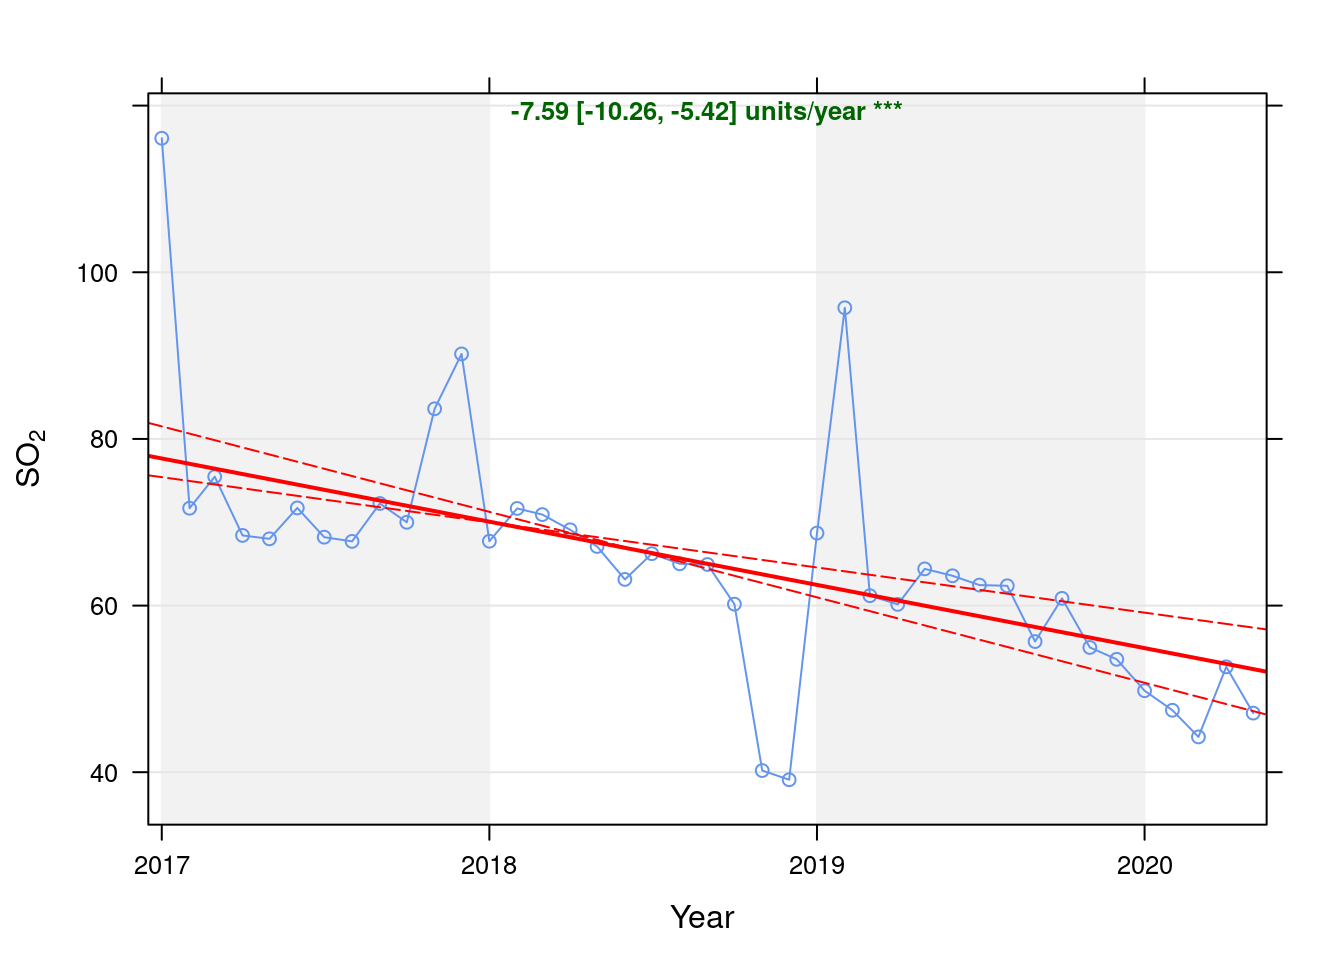
\includegraphics{/home/ba1e12/github/dataknut/airQual/docs/sccAirQualExplore_covidLockdown2020ForBBCsnaphot_files/figure-latex/theilSenSO2-1.pdf}
\caption{(\#fig:theilSenSO2)Theil-Sen trend (SO2)}
\end{figure}

\begin{Shaded}
\begin{Highlighting}[]
\NormalTok{t <-}\StringTok{ }\KeywordTok{getModelTrendTable}\NormalTok{(oaSO2, }\DataTypeTok{fname =} \StringTok{"SO2"}\NormalTok{)}

\NormalTok{ft <-}\StringTok{ }\KeywordTok{dcast}\NormalTok{(t[date }\OperatorTok{>=}\StringTok{ }\KeywordTok{as.Date}\NormalTok{(}\StringTok{"2020-01-01"}\NormalTok{) }\OperatorTok{&}\StringTok{ }\NormalTok{date }\OperatorTok{<}\StringTok{ }\KeywordTok{as.Date}\NormalTok{(}\StringTok{"2020-06-01"}\NormalTok{)], date }\OperatorTok{~}\StringTok{ }\NormalTok{., }\DataTypeTok{value.var =} \KeywordTok{c}\NormalTok{(}\StringTok{"diff"}\NormalTok{, }\StringTok{"pcDiff"}\NormalTok{))}
\NormalTok{ft[, }\StringTok{`}\DataTypeTok{:=}\StringTok{`}\NormalTok{(date, }\KeywordTok{format.Date}\NormalTok{(date, }\DataTypeTok{format =} \StringTok{"%b %Y"}\NormalTok{))]}
\NormalTok{kableExtra}\OperatorTok{::}\KeywordTok{kable}\NormalTok{(ft, }\DataTypeTok{caption =} \StringTok{"Units and % above/below expected"}\NormalTok{, }\DataTypeTok{digits =} \DecValTok{2}\NormalTok{) }\OperatorTok\StringTok{ }\KeywordTok{kable_styling}\NormalTok{()}
\end{Highlighting}
\end{Shaded}

(\#tab:theilSenSO2)Units and \% above/below expected

date

diff

pcDiff

Jan 2020

-5.11

-9.30

Feb 2020

-6.81

-12.55

Mar 2020

-9.41

-17.54

Apr 2020

-0.35

-0.66

May 2020

-5.28

-10.08

\section{Ozone}\label{ozone}

\begin{Shaded}
\begin{Highlighting}[]
\NormalTok{yLab <-}\StringTok{ "Ozone (ug/m3)"}
\NormalTok{o3dt <-}\StringTok{ }\NormalTok{fixedDT[pollutant }\OperatorTok{==}\StringTok{ "o3"}\NormalTok{]}
\end{Highlighting}
\end{Shaded}

Figure @ref(fig:theilSenO3) shows the O3 trend over time. Is lockdown
below trend?

\begin{Shaded}
\begin{Highlighting}[]
\NormalTok{o3dt[, }\StringTok{`}\DataTypeTok{:=}\StringTok{`}\NormalTok{(date, }\KeywordTok{as.Date}\NormalTok{(dateTimeUTC))]  }\CommentTok{# set date to date for this one}

\NormalTok{oaO3 <-}\StringTok{ }\NormalTok{openair}\OperatorTok{::}\KeywordTok{TheilSen}\NormalTok{(o3dt[date }\OperatorTok{<}\StringTok{ }\KeywordTok{as.Date}\NormalTok{(}\StringTok{"2020-06-01"}\NormalTok{)], }\StringTok{"value"}\NormalTok{, }\DataTypeTok{ylab =} \StringTok{"O3"}\NormalTok{, }\DataTypeTok{deseason =} \OtherTok{TRUE}\NormalTok{, }\DataTypeTok{xlab =} \StringTok{"Year"}\NormalTok{, }
    \DataTypeTok{date.format =} \StringTok{"%Y"}\NormalTok{, }\DataTypeTok{date.breaks =} \DecValTok{4}\NormalTok{)}
\end{Highlighting}
\end{Shaded}

\begin{verbatim}
## [1] "Taking bootstrap samples. Please wait."
\end{verbatim}

\begin{figure}
\centering
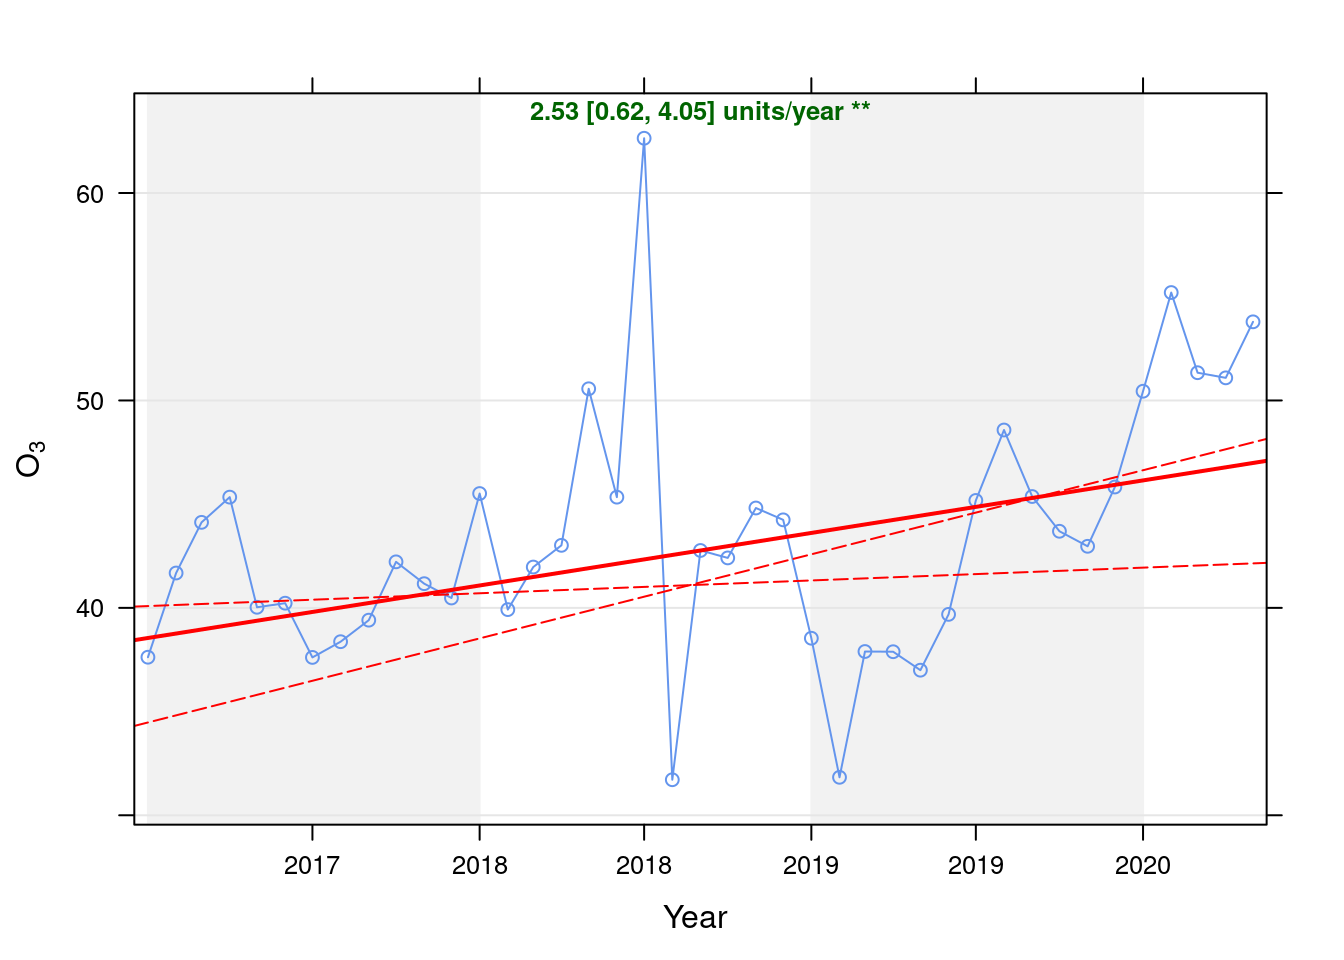
\includegraphics{/home/ba1e12/github/dataknut/airQual/docs/sccAirQualExplore_covidLockdown2020ForBBCsnaphot_files/figure-latex/theilSenO3-1.pdf}
\caption{(\#fig:theilSenO3)Theil-Sen trend (O3)}
\end{figure}

\begin{Shaded}
\begin{Highlighting}[]
\NormalTok{t <-}\StringTok{ }\KeywordTok{getModelTrendTable}\NormalTok{(oaO3, }\DataTypeTok{fname =} \StringTok{"O3"}\NormalTok{)}

\NormalTok{ft <-}\StringTok{ }\KeywordTok{dcast}\NormalTok{(t[date }\OperatorTok{>=}\StringTok{ }\KeywordTok{as.Date}\NormalTok{(}\StringTok{"2020-01-01"}\NormalTok{) }\OperatorTok{&}\StringTok{ }\NormalTok{date }\OperatorTok{<}\StringTok{ }\KeywordTok{as.Date}\NormalTok{(}\StringTok{"2020-06-01"}\NormalTok{)], date }\OperatorTok{~}\StringTok{ }\NormalTok{., }\DataTypeTok{value.var =} \KeywordTok{c}\NormalTok{(}\StringTok{"diff"}\NormalTok{, }\StringTok{"pcDiff"}\NormalTok{))}
\NormalTok{ft[, }\StringTok{`}\DataTypeTok{:=}\StringTok{`}\NormalTok{(date, }\KeywordTok{format.Date}\NormalTok{(date, }\DataTypeTok{format =} \StringTok{"%b %Y"}\NormalTok{))]}
\NormalTok{kableExtra}\OperatorTok{::}\KeywordTok{kable}\NormalTok{(ft, }\DataTypeTok{caption =} \StringTok{"Units and % above/below expected"}\NormalTok{, }\DataTypeTok{digits =} \DecValTok{2}\NormalTok{) }\OperatorTok\StringTok{ }\KeywordTok{kable_styling}\NormalTok{()}
\end{Highlighting}
\end{Shaded}

(\#tab:theilSenO3)Units and \% above/below expected

date

diff

pcDiff

Jan 2020

4.30

9.31

Feb 2020

8.84

19.07

Mar 2020

4.77

10.25

Apr 2020

4.31

9.22

May 2020

6.80

14.48

\section{PM 10}\label{pm-10}

\begin{Shaded}
\begin{Highlighting}[]
\NormalTok{yLab <-}\StringTok{ "PM 10 (ug/m3)"}
\NormalTok{pm10dt <-}\StringTok{ }\NormalTok{fixedDT[pollutant }\OperatorTok{==}\StringTok{ "pm10"}\NormalTok{]}
\end{Highlighting}
\end{Shaded}

Figure @ref(fig:theilSenPM10) shows the PM10 trend over time. Is
lockdown below trend?

\begin{Shaded}
\begin{Highlighting}[]
\NormalTok{pm10dt[, }\StringTok{`}\DataTypeTok{:=}\StringTok{`}\NormalTok{(date, }\KeywordTok{as.Date}\NormalTok{(dateTimeUTC))]  }\CommentTok{# set date to date for this one}

\NormalTok{oaPM10 <-}\StringTok{ }\NormalTok{openair}\OperatorTok{::}\KeywordTok{TheilSen}\NormalTok{(pm10dt[date }\OperatorTok{<}\StringTok{ }\KeywordTok{as.Date}\NormalTok{(}\StringTok{"2020-06-01"}\NormalTok{)], }\StringTok{"value"}\NormalTok{, }\DataTypeTok{ylab =} \StringTok{"PM10"}\NormalTok{, }\DataTypeTok{deseason =} \OtherTok{TRUE}\NormalTok{, }\DataTypeTok{xlab =} \StringTok{"Year"}\NormalTok{, }
    \DataTypeTok{date.format =} \StringTok{"%Y"}\NormalTok{, }\DataTypeTok{date.breaks =} \DecValTok{4}\NormalTok{)}
\end{Highlighting}
\end{Shaded}

\begin{verbatim}
## [1] "Taking bootstrap samples. Please wait."
\end{verbatim}

\begin{figure}
\centering
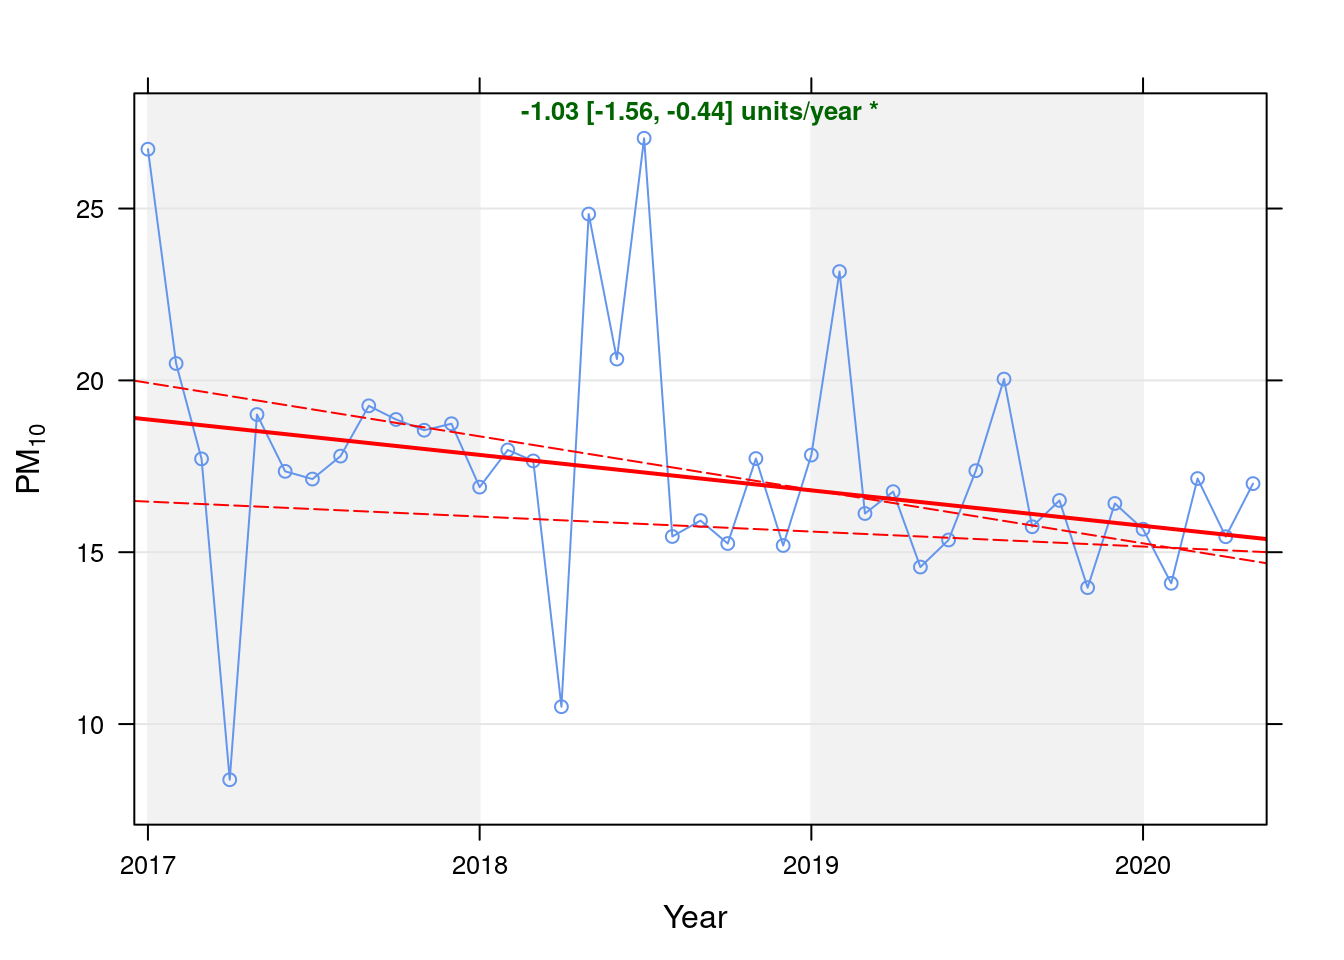
\includegraphics{/home/ba1e12/github/dataknut/airQual/docs/sccAirQualExplore_covidLockdown2020ForBBCsnaphot_files/figure-latex/theilSenPM10-1.pdf}
\caption{(\#fig:theilSenPM10)Theil-Sen trend (PM10)}
\end{figure}

\begin{Shaded}
\begin{Highlighting}[]
\NormalTok{t <-}\StringTok{ }\KeywordTok{getModelTrendTable}\NormalTok{(oaPM10, }\DataTypeTok{fname =} \StringTok{"SPM10"}\NormalTok{)}

\NormalTok{ft <-}\StringTok{ }\KeywordTok{dcast}\NormalTok{(t[date }\OperatorTok{>=}\StringTok{ }\KeywordTok{as.Date}\NormalTok{(}\StringTok{"2020-01-01"}\NormalTok{) }\OperatorTok{&}\StringTok{ }\NormalTok{date }\OperatorTok{<}\StringTok{ }\KeywordTok{as.Date}\NormalTok{(}\StringTok{"2020-06-01"}\NormalTok{)], date }\OperatorTok{~}\StringTok{ }\NormalTok{., }\DataTypeTok{value.var =} \KeywordTok{c}\NormalTok{(}\StringTok{"diff"}\NormalTok{, }\StringTok{"pcDiff"}\NormalTok{))}
\NormalTok{ft[, }\StringTok{`}\DataTypeTok{:=}\StringTok{`}\NormalTok{(date, }\KeywordTok{format.Date}\NormalTok{(date, }\DataTypeTok{format =} \StringTok{"%b %Y"}\NormalTok{))]}
\NormalTok{kableExtra}\OperatorTok{::}\KeywordTok{kable}\NormalTok{(ft, }\DataTypeTok{caption =} \StringTok{"Units and % above/below expected"}\NormalTok{, }\DataTypeTok{digits =} \DecValTok{2}\NormalTok{) }\OperatorTok\StringTok{ }\KeywordTok{kable_styling}\NormalTok{()}
\end{Highlighting}
\end{Shaded}

(\#tab:theilSenPM10)Units and \% above/below expected

date

diff

pcDiff

Jan 2020

-0.10

-0.62

Feb 2020

-1.58

-10.10

Mar 2020

1.55

9.91

Apr 2020

-0.06

-0.38

May 2020

1.57

10.19

\section{PM 2.5}\label{pm-2.5}

\begin{Shaded}
\begin{Highlighting}[]
\NormalTok{yLab <-}\StringTok{ "PM 2.5 (ug/m3)"}
\NormalTok{pm25dt <-}\StringTok{ }\NormalTok{fixedDT[pollutant }\OperatorTok{==}\StringTok{ "pm2.5"}\NormalTok{]}
\end{Highlighting}
\end{Shaded}

Figure @ref(fig:theilSenPM25) shows the PM10 trend over time. Is
lockdown below trend?

\begin{Shaded}
\begin{Highlighting}[]
\NormalTok{pm25dt[, }\StringTok{`}\DataTypeTok{:=}\StringTok{`}\NormalTok{(date, }\KeywordTok{as.Date}\NormalTok{(dateTimeUTC))]  }\CommentTok{# set date to date for this one}

\NormalTok{oaPM25 <-}\StringTok{ }\NormalTok{openair}\OperatorTok{::}\KeywordTok{TheilSen}\NormalTok{(pm25dt[date }\OperatorTok{<}\StringTok{ }\KeywordTok{as.Date}\NormalTok{(}\StringTok{"2020-06-01"}\NormalTok{)], }\StringTok{"value"}\NormalTok{, }\DataTypeTok{ylab =} \StringTok{"PM2.5"}\NormalTok{, }\DataTypeTok{deseason =} \OtherTok{TRUE}\NormalTok{, }\DataTypeTok{xlab =} \StringTok{"Year"}\NormalTok{, }
    \DataTypeTok{date.format =} \StringTok{"%Y"}\NormalTok{, }\DataTypeTok{date.breaks =} \DecValTok{4}\NormalTok{)}
\end{Highlighting}
\end{Shaded}

\begin{verbatim}
## [1] "Taking bootstrap samples. Please wait."
\end{verbatim}

\begin{figure}
\centering
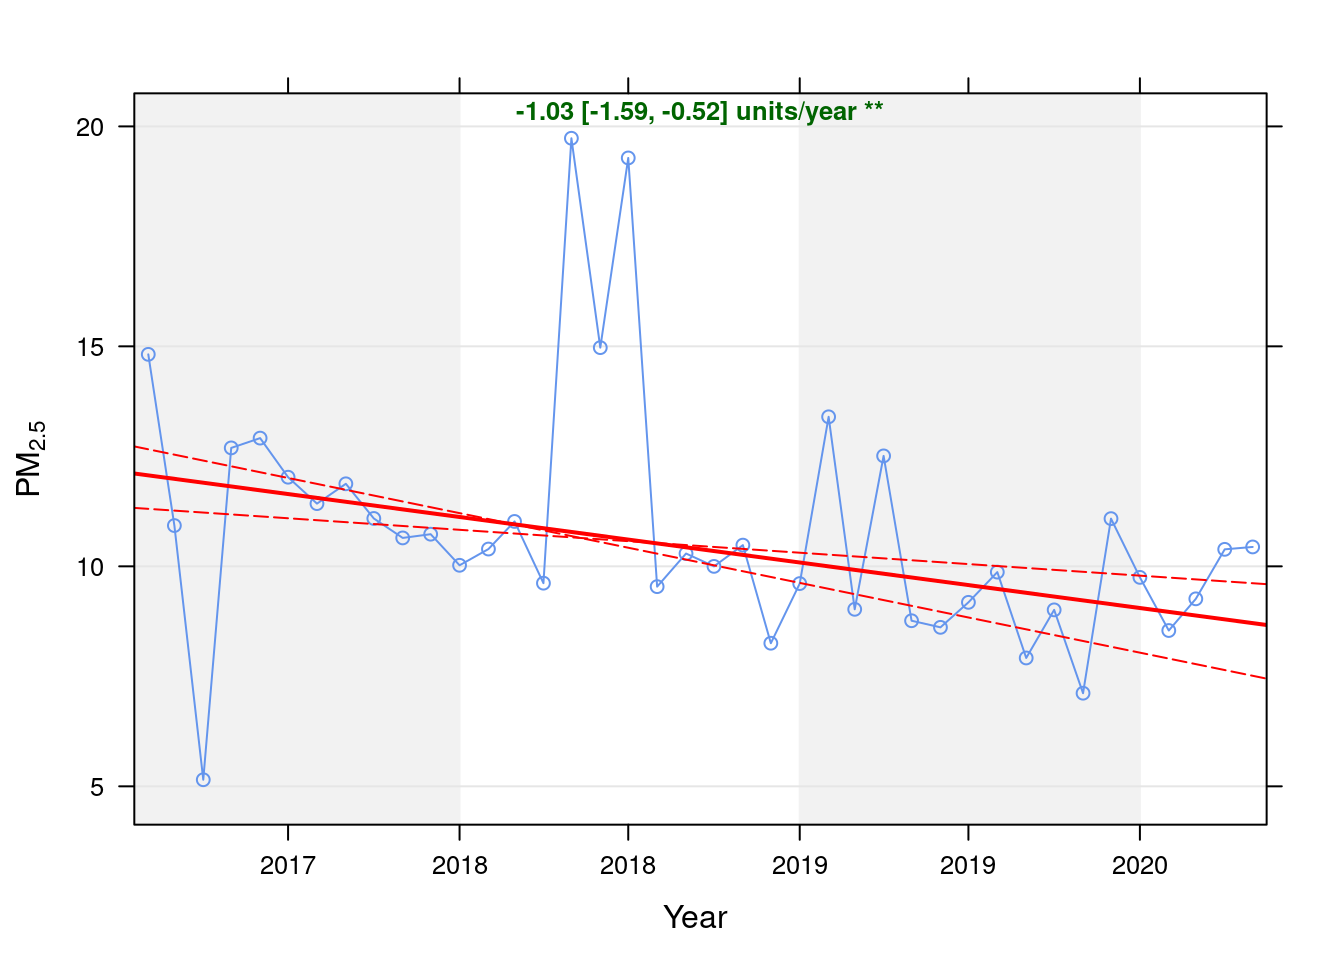
\includegraphics{/home/ba1e12/github/dataknut/airQual/docs/sccAirQualExplore_covidLockdown2020ForBBCsnaphot_files/figure-latex/theilSenPM25-1.pdf}
\caption{(\#fig:theilSenPM25)Theil-Sen trend (PM2.5)}
\end{figure}

\begin{Shaded}
\begin{Highlighting}[]
\NormalTok{t <-}\StringTok{ }\KeywordTok{getModelTrendTable}\NormalTok{(oaPM25, }\DataTypeTok{fname =} \StringTok{"PM2.5"}\NormalTok{)}

\NormalTok{ft <-}\StringTok{ }\KeywordTok{dcast}\NormalTok{(t[date }\OperatorTok{>=}\StringTok{ }\KeywordTok{as.Date}\NormalTok{(}\StringTok{"2020-01-01"}\NormalTok{) }\OperatorTok{&}\StringTok{ }\NormalTok{date }\OperatorTok{<}\StringTok{ }\KeywordTok{as.Date}\NormalTok{(}\StringTok{"2020-06-01"}\NormalTok{)], date }\OperatorTok{~}\StringTok{ }\NormalTok{., }\DataTypeTok{value.var =} \KeywordTok{c}\NormalTok{(}\StringTok{"diff"}\NormalTok{, }\StringTok{"pcDiff"}\NormalTok{))}
\NormalTok{ft[, }\StringTok{`}\DataTypeTok{:=}\StringTok{`}\NormalTok{(date, }\KeywordTok{format.Date}\NormalTok{(date, }\DataTypeTok{format =} \StringTok{"%b %Y"}\NormalTok{))]}
\NormalTok{kableExtra}\OperatorTok{::}\KeywordTok{kable}\NormalTok{(ft, }\DataTypeTok{caption =} \StringTok{"Units and % above/below expected"}\NormalTok{, }\DataTypeTok{digits =} \DecValTok{2}\NormalTok{) }\OperatorTok\StringTok{ }\KeywordTok{kable_styling}\NormalTok{()}
\end{Highlighting}
\end{Shaded}

(\#tab:theilSenPM25)Units and \% above/below expected

date

diff

pcDiff

Jan 2020

0.70

7.70

Feb 2020

-0.42

-4.72

Mar 2020

0.38

4.27

Apr 2020

1.59

18.11

May 2020

1.73

19.89

\section{About}\label{about}

\subsection{Code}\label{code}

Source:

\begin{itemize}
\tightlist
\item
  \url{https://github.com/dataknut/airQual}
\end{itemize}

History:

\begin{itemize}
\tightlist
\item
  \url{https://github.com/dataknut/airQual/commits/master}
\end{itemize}

\subsection{Comments and feedback}\label{comments-and-feedback}

If you wish to comment please open an issue:

\begin{itemize}
\tightlist
\item
  \url{https://github.com/dataknut/airQual/issues}
\end{itemize}

\subsection{Citation}\label{citation}

If you wish to refer to any of the material from this report please cite
as:

\begin{itemize}
\tightlist
\item
  Anderson, B., (2020) Air Quality in Southampton (UK): Exploring the
  effect of UK covid 19 lockdown on air quality: Summary for BBC South ,
  \href{http://www.energy.soton.ac.uk}{Sustainable Energy Research
  Group}, University of Southampton: Southampton, UK.
\end{itemize}

Report circulation:

\begin{itemize}
\tightlist
\item
  Public
\end{itemize}

This work is (c) 2020 the University of Southampton and is part of a
collection of \href{https://dataknut.github.io/airQual/}{air quality}
data analyses.

\section{Runtime}\label{runtime}

Report generated using
\href{https://cran.r-project.org/package=knitr}{knitr} in
\href{http://www.rstudio.com}{RStudio} with R version 3.6.0 (2019-04-26)
running on x86\_64-redhat-linux-gnu (\#1 SMP Thu May 7 19:30:37 EDT
2020).

\begin{Shaded}
\begin{Highlighting}[]
\NormalTok{t <-}\StringTok{ }\KeywordTok{proc.time}\NormalTok{() }\OperatorTok{-}\StringTok{ }\NormalTok{myParams}\OperatorTok{$}\NormalTok{startTime}

\NormalTok{elapsed <-}\StringTok{ }\NormalTok{t[[}\DecValTok{3}\NormalTok{]]}
\end{Highlighting}
\end{Shaded}

Analysis completed in 13.226 seconds ( 0.22 minutes).

R packages used in this report:

\begin{itemize}
\tightlist
\item
  data.table - (Dowle et al. 2015)
\item
  ggplot2 - (Wickham 2009)
\item
  here - (Müller 2017)
\item
  kableExtra - (Zhu 2019)
\item
  lubridate - (Grolemund and Wickham 2011)
\item
  openAir - (Carslaw and Ropkins 2012)
\item
  skimr - (Arino de la Rubia et al. 2017)
\item
  viridis - (Garnier 2018)
\end{itemize}

\section*{References}\label{references}
\addcontentsline{toc}{section}{References}

\hypertarget{refs}{}
\hypertarget{ref-skimr}{}
Arino de la Rubia, Eduardo, Hao Zhu, Shannon Ellis, Elin Waring, and
Michael Quinn. 2017. \emph{Skimr: Skimr}.
\url{https://github.com/ropenscilabs/skimr}.

\hypertarget{ref-openair}{}
Carslaw, David C., and Karl Ropkins. 2012. ``Openair --- an R Package
for Air Quality Data Analysis.'' \emph{Environmental Modelling \&
Software} 27--28 (0): 52--61.
doi:\href{https://doi.org/10.1016/j.envsoft.2011.09.008}{10.1016/j.envsoft.2011.09.008}.

\hypertarget{ref-data.table}{}
Dowle, M, A Srinivasan, T Short, S Lianoglou with contributions from R
Saporta, and E Antonyan. 2015. \emph{Data.table: Extension of
Data.frame}. \url{https://CRAN.R-project.org/package=data.table}.

\hypertarget{ref-viridis}{}
Garnier, Simon. 2018. \emph{Viridis: Default Color Maps from
'Matplotlib'}. \url{https://CRAN.R-project.org/package=viridis}.

\hypertarget{ref-lubridate}{}
Grolemund, Garrett, and Hadley Wickham. 2011. ``Dates and Times Made
Easy with lubridate.'' \emph{Journal of Statistical Software} 40 (3):
1--25. \url{http://www.jstatsoft.org/v40/i03/}.

\hypertarget{ref-here}{}
Müller, Kirill. 2017. \emph{Here: A Simpler Way to Find Your Files}.
\url{https://CRAN.R-project.org/package=here}.

\hypertarget{ref-ggplot2}{}
Wickham, Hadley. 2009. \emph{Ggplot2: Elegant Graphics for Data
Analysis}. Springer-Verlag New York. \url{http://ggplot2.org}.

\hypertarget{ref-kableExtra}{}
Zhu, Hao. 2019. \emph{KableExtra: Construct Complex Table with 'Kable'
and Pipe Syntax}. \url{https://CRAN.R-project.org/package=kableExtra}.

\end{document}
